% TODO fix pagebreaks
\documentclass[12pt,a4paper]{article}
\usepackage[utf8]{inputenc}
\usepackage[margin=1in,headheight=15pt]{geometry}
\usepackage{amsmath,amssymb,amsfonts}
\usepackage{graphicx}
\usepackage{cite}
\usepackage{hyperref}
\usepackage{booktabs}
\usepackage{tabularx}
\usepackage{tikz}
\usetikzlibrary{shapes.geometric, arrows, arrows.meta, positioning, calc, fit, backgrounds, matrix, shadows, shapes.multipart}
\usepackage{setspace}
\usepackage{fancyhdr}

% Line spacing
\onehalfspacing

% Hyperref setup
\hypersetup{
    colorlinks=true,
    linkcolor=black,
    filecolor=black,      
    urlcolor=blue,
    citecolor=black,
}

% TikZ Styles for Flowcharts & Diagrams
\tikzset{
    startstop/.style={rectangle, rounded corners, minimum width=2.5cm, minimum height=0.8cm, text centered, draw=black, fill=blue!10, font=\small},
    process/.style={rectangle, minimum width=2.5cm, minimum height=0.8cm, text centered, draw=black, fill=orange!10, font=\small},
    decision/.style={diamond, minimum width=2cm, minimum height=0.8cm, text centered, draw=black, fill=green!10, aspect=2, font=\small},
    arrow/.style={thick,->,>=stealth}
}

\begin{document}

%===========================================================
% TITLE PAGE
%===========================================================
\begin{titlepage}
    \begin{center}
        \vspace*{0.5cm}
        
        {\large \textbf{SYNOPSIS OF THE B.TECH PROJECT ENTITLED}} \\[0.5cm]
        \hrule
        \vspace{0.4cm}
        {\Large \textbf{DESIGN AND DEVELOPMENT OF A SELF-CORRECTING RETRIEVAL-AUGMENTED GENERATION (RAG) SYSTEM}} \\
        \vspace{0.4cm}
        \hrule
        \vspace{1.5cm}
        
        {\large A synopsis Submitted \\ In Partial Fulfillment of the Requirements \\ for the Degree of} \\[0.5cm]
        {\Large \textbf{BACHELOR OF TECHNOLOGY}} \\
        {\large (Computer Science \& Engineering)} \\[1.5cm]
        
        \textbf{By} \\[0.5cm]
        \begin{tabular}{cc}
            \textbf{Student Name} & \textbf{Enrollment Number} \\
            \midrule
            Manas Khanna & A25305223002 \\
            Gurmukh Singh & A25305223008 \\
            Arshleen Kaur & A25305223141 \\
        \end{tabular} \\[1.5cm]
        
        \textbf{Under the Supervision of} \\[0.3cm]
        {\large \textbf{Dr. Gurpreet Singh}} \\
        {Assistant Professor} \\[1.5cm]
        
        \vfill
        
        \begin{figure}[h]
            \centering
            
\includegraphics[width=3cm]{images/Amity.png}
        \end{figure}
        
        {\large \textbf{AMITY UNIVERSITY PUNJAB, INDIA}} \\
        {\large July, 2026}
        
    \end{center}
\end{titlepage}

\newpage
\pagenumbering{roman}

%===========================================================
% DECLARATION
%===========================================================
\section*{Declaration}
\addcontentsline{toc}{section}{Declaration}
We hereby declare that this SYNOPSIS report entitled, ``\textbf{Design and Development of a Self-Correcting Retrieval-Augmented Generation (RAG) System}'', being submitted by us to \textbf{Amity University Punjab} for the award of the degree of Bachelor of Technology (Computer Science \& Engineering) is a record of bonafide work carried by us. We worked under the guidance and supervision of \textbf{Dr. Gurpreet Singh, Assistant Professor}.

The matter embodied in this report has not been submitted to any other university or institute earlier for the award of any degree or diploma.

\vspace{2.5cm}

\noindent
\begin{tabularx}{\textwidth}{XXX}
    \textbf{Manas Khanna} & \textbf{Gurmukh Singh} & \textbf{Arshleen Kaur} \\
    B. TECH. Sem VII & B. TECH. Sem VII & B. TECH. Sem VII \\
    (Session 2023-2027) & (Session 2023-2027) & (Session 2023-2027) \\
    Roll No: A25305223002 & Roll No: A25305223008 & Roll No: A25305223141
\end{tabularx}

\newpage

%===========================================================
% ACKNOWLEDGEMENTS
%===========================================================
\section*{Acknowledgements}
\addcontentsline{toc}{section}{Acknowledgements}
We have taken efforts in this project. However, it would not have been possible without the kind support and help of many individuals and organizations. We would like to extend our sincere thanks to all of them.

We would like to take the opportunity to express our humble gratitude to \textbf{Dr. Gurpreet Singh, Assistant Professor}, under whom we executed this project, and are most thankful for his constant guidance and willingness to share his vast knowledge which made us understand this project and its manifestation in great depth and helped us to complete the assigned task.

\vspace{3cm}

\noindent
\textbf{PLACE:} Mohali, India \\
\textbf{DATE:} July 2026

\vspace{1.5cm}

\noindent
\begin{tabularx}{\textwidth}{XXX}
    \rule{3.5cm}{0.4pt} & \rule{3.5cm}{0.4pt} & \rule{3.5cm}{0.4pt} \\
    \textbf{Manas Khanna} & \textbf{Gurmukh Singh} & \textbf{Arshleen Kaur} \\
    Roll No: A25305223002 & Roll No: A25305223008 & Roll No: A25305223141
\end{tabularx}

\newpage

%===========================================================
% TABLE OF CONTENTS
%===========================================================
\renewcommand{\contentsname}{CONTENT}
\tableofcontents

\newpage
\pagenumbering{arabic}

%===========================================================
% ABSTRACT (TOC starts here)
%===========================================================
\section*{Abstract}
\addcontentsline{toc}{section}{Abstract}
Large Language Models (LLMs) have demonstrated exceptional capabilities in natural language understanding and text generation. However, they frequently suffer from factuality errors and hallucinations due to their reliance on static parametric knowledge. Retrieval-Augmented Generation (RAG) mitigates this by integrating external vector search. Nonetheless, standard RAG systems act as passive consumers of retrieved information, leaving them vulnerable to poor-quality retrievals, noise, and hallucinations if the retrieved documents are irrelevant. 

This project proposes a \textbf{Self-Correcting Retrieval-Augmented Generation (Self-Correcting RAG)} system. The framework extends the Corrective Retrieval-Augmented Generation (CRAG) model by introducing a secondary self-evaluation and reflection module. A lightweight retrieval evaluator assesses retrieved document relevance, dynamically triggering knowledge refinement, web search augmentation, or query rewriting based on three confidence states: Correct, Ambiguous, and Incorrect. Following generation, a self-reflection loop critiques the answer's groundedness, completeness, and hallucination status, triggering iterative context expansion or answer regeneration if required. This system aims to provide robust, factual, and verified responses for knowledge-intensive question-answering tasks.

\newpage

%===========================================================
% 1. INTRODUCTION
%===========================================================
\section{Introduction}
Large Language Models (LLMs) have transformed natural language processing. Despite their success, LLMs encounter factual errors, particularly when answering queries requiring specific, real-time, or long-tail knowledge. Retrieval-Augmented Generation (RAG) addresses this by fetching documents from an external corpus to aid the LLM. 

Despite the benefits of RAG, standard implementations suffer from three critical challenges:
\begin{enumerate}
    \item \textbf{Retrieval Failure:} If the retriever fetches irrelevant or noisy documents, the generator is misled, leading to incorrect answers.
    \item \textbf{Redundant Context:} Complete documents are often fed to the generator, introducing clutter and exceeding the LLM's optimal context length.
    \item \textbf{Absence of Post-Generation Reflection:} The generator produces responses in a single forward pass without validating if the response is supported by the retrieved context.
\end{enumerate}

To overcome these limits, this project presents a Self-Correcting RAG system. It introduces a two-tier evaluation mechanism: a \textit{Pre-generation Retrieval Evaluator} that corrects retrieved contexts using internal refinement and external web search, and a \textit{Post-generation Reflection Module} that evaluates the generated output for groundedness and completeness.

\subsection{Literature Review}
The evolution of knowledge-augmented generation spans several milestones:
\begin{itemize}
    \item \textbf{Standard RAG (Lewis et al., 2020):} Introduced the framework coupling dense vector retrieval (e.g., DPR) with an encoder-decoder generator. It relies on the assumption that retrieved documents are always high-quality and relevant.
    \item \textbf{Self-RAG (Asai et al., 2024):} Proposed instruction-tuning LLMs with special ``critique tokens'' to decide when to retrieve and self-evaluate responses. Although powerful, Self-RAG requires fine-tuning large models (e.g., LLaMA-2 7B/13B), which is computationally expensive and complex to generalize across arbitrary LLMs.
    \item \textbf{Corrective RAG (CRAG) (Yan et al., 2024):} Introduced a lightweight retrieval evaluator (0.77B T5-large) that classifies retrieved relevance into \textit{Correct}, \textit{Incorrect}, and \textit{Ambiguous}. It triggers web-search queries for incorrect/ambiguous cases and performs a decompose-then-recompose step on document segments to strip out noisy text.
\end{itemize}
Our project builds on the plug-and-play architecture of CRAG and integrates an orchestrator-driven self-correction feedback loop. Unlike CRAG, which assumes the generator output is final, our system adds a verification layer that critiques the response against the refined context, allowing self-corrective iterations before final delivery.

\newpage

%===========================================================
% 2. SCOPE & OBJECTIVE OF THE PROJECT
%===========================================================
\section{Scope and Objective of the Project}

\subsection{Project Scope}
The scope of this project lies in designing and building a state-of-the-art framework for context-grounded text generation that functions as an intelligent, self-correcting agent. Specifically, it involves:
\begin{enumerate}
    \item Structuring an ingestion pipeline that handles diverse text documents, builds vector index databases, and runs local dense retrievers.
    \item Integrating a lightweight evaluator model that calculates relevance scores and outputs a routing state (Correct, Incorrect, or Ambiguous).
    \item Constructing fallback pathways to query public search APIs for real-time information retrieval when the internal corpus is insufficient.
    \item Designing an LLM-based critique module that scores generated responses for factual groundedness, relevance, and query coverage.
    \begin{equation*}
        \text{Relevance Score} = f(\text{Retrieved Docs}, \text{Query})
    \end{equation*}
    \item Orchestrating these components as a directed graph using LangGraph to enable cyclical feedback loops.
\end{enumerate}

\subsection{Project Objectives}
Given a user query $x$ and a document corpus $\mathcal{C}$, standard RAG systems generate an answer $y$ by directly feeding the retrieved documents $\mathcal{D}$ to the LLM generator. When $\mathcal{D}$ contains irrelevant information, the system fails. The objective is to design a self-correcting pipeline that:
\begin{enumerate}
    \item Evaluates the quality of retrieved documents $\mathcal{D}$ before generation.
    \item Refines or replaces $\mathcal{D}$ dynamically using document stripping or web search.
    \item Critiques the generated answer $y$ post-generation to check for hallucinations and incompleteness, regenerating the answer if confidence is low.
\end{enumerate}

Formally, the retrieved documents are represented as:
\begin{equation*}
    \mathcal{D} = \{d_1, d_2, \dots, d_k\} \subset \mathcal{C}
\end{equation*}
The pre-evaluation score maps to a confidence state $S$:
\begin{equation*}
    S = \text{Evaluator}(x, \mathcal{D}) \in \{\text{Correct}, \text{Incorrect}, \text{Ambiguous}\}
\end{equation*}
For generating response $y$, the generator uses refined context $K$:
\begin{equation*}
    y = \text{LLM}(x, K)
\end{equation*}
Where the post-generation module validates the response by evaluating groundedness against the context:
\begin{equation*}
    \text{Groundedness}(y, K) \to \{\text{Entailed}, \text{Hallucinated}\}
\end{equation*}

\newpage

%===========================================================
% 3. ROLES AND RESPONSIBILITIES
%===========================================================
\section{Roles and Responsibilities}
This project is a collaborative effort by the team members. To ensure efficient execution and integration, the project responsibilities are divided into major modules: Ingestion and Retrieval, Relevance Evaluation and Search Augmentation, and Critique Agents and Orchestration. 

The development responsibilities are distributed as follows:
\begin{itemize}
    \item \textbf{Module 1: Data Ingestion and Retrieval System} \\
    Focuses on raw document processing, text splitting, metadata extraction, embedding generation, and indexing in the vector database. It ensures high-quality embedding representation of the internal knowledge base.
    
    \item \textbf{Module 2: Pre-generation Evaluation and Query Rewriting} \\
    Handles the confidence-based relevance assessment of retrieved documents, query extraction, and external API search query generation. It is responsible for formatting documents into concise knowledge strips.
    
    \item \textbf{Module 3: Post-generation Reflection and Graph Orchestration} \\
    Orchestrates the overall workflow using state-machine routing, executes the LLM generator, evaluates the generated output for groundedness and completeness, and manages the cyclical feedback loop.
\end{itemize}

All team members jointly participate in system integration, model evaluation, testing, benchmarking, and documentation.

\newpage

%===========================================================
% 4. REQUIREMENTS ANALYSIS
%===========================================================
\section{Requirements Analysis}
To develop a robust and effective Self-Correcting RAG system, the system requirements are categorized into functional and non-functional requirements:

\subsection{Functional Requirements}
\begin{enumerate}
    \item \textbf{Vector Database Setup:} The system must load, chunk, embed, and store document corpora in ChromaDB/FAISS.
    \item \textbf{Dense Retrieval:} The system must accept user queries and retrieve the top-$k$ relevant documents.
    \item \textbf{Relevance Evaluation:} A retrieval evaluator must assess the relevance of each document and classify the state into Correct, Ambiguous, or Incorrect.
    \item \textbf{Web Search Fallback:} If the evaluation state is Incorrect or Ambiguous, the system must trigger query rewriting and perform web search queries to fetch external documents.
    \item \textbf{Context Refinement:} Relevant retrieved context must be stripped of noise and formatted into concise knowledge strips.
    \item \textbf{Answer Generation:} The LLM generator must generate responses using only the refined context.
    \item \textbf{Post-Generation Reflection:} The feedback module must check the generated answer for groundedness (hallucinations) and query coverage, and trigger regeneration if necessary.
\end{enumerate}

\subsection{Non-Functional Requirements}
\begin{enumerate}
    \item \textbf{Accuracy and Faithfulness:} Responses must be highly faithful to the context, minimizing hallucinations.
    \item \textbf{Performance and Latency:} The average processing time for a query (including retrieval, evaluation, search, and generation) must be optimized.
    \item \textbf{Modularity:} The architecture must allow easy swap-in/swap-out of different embedding models or generators.
    \item \textbf{Reliability:} The system must handle search API failures or model timeouts gracefully.
\end{enumerate}

\newpage

%===========================================================
% 5. SOFTWARE SPECIFICATION
%===========================================================
\section{Software Specification}
The software specification stack defined for the implementation of the Self-Correcting RAG project is shown in Table \ref{tab:software_specs}.

\begin{table}[h!]
    \centering
    \small
    \begin{tabularx}{\textwidth}{lX}
        \toprule
        \textbf{Specification Item} & \textbf{Details} \\
        \midrule
        \textbf{Operating System} & Arch Linux / Windows 11 \\
        \textbf{IDE \& Development Tools} & Neovim / VS Code \\
        \textbf{Versioning System} & Git \& GitHub \\
        \textbf{Database} & ChromaDB (Vector DB) \& SQLite3 (State Store) \\
        \textbf{Web Server} & FastAPI (Backend API) \\
        \textbf{Languages \& Frameworks} & Python 3.10+, LangGraph, LangChain \\
        \bottomrule
    \end{tabularx}
    \caption{Software Specifications.}
    \label{tab:software_specs}
\end{table}

\newpage

%===========================================================
% 6. SYSTEM DESIGN/ METHODOLOGY
%===========================================================
\section{System Design and Methodology}
The proposed Self-Correcting RAG system is designed around an orchestrated workflow using LangGraph state machines. The detailed flow of the system is shown in Figure \ref{fig:architecture}.

The system operates in four stages:
\begin{enumerate}
    \item \textbf{Retrieval Stage:} Given a query $x$, the top-$k$ documents are retrieved. The evaluator scores the documents. Let $s_i$ be the relevance score of document $d_i$.
    \item \textbf{Evaluator Stage:} Classification of document relevance.
    \begin{itemize}
        \item \textbf{Correct:} If $\max(s_i) \geq T_{high}$, the documents are refined using document splitting into sentence-level strips. Low-relevance strips are filtered out.
        \item \textbf{Incorrect:} If $\max(s_i) < T_{low}$, the documents are discarded. A query rewriter $W$ extracts search keywords, and a Web Search API fetches external context.
        \item \textbf{Ambiguous:} If $T_{low} \leq \max(s_i) < T_{high}$, internal documents are refined and combined with web search results.
    \end{itemize}
    \item \textbf{Generation Stage:} The LLM generator produces an initial answer $A_0$ from the refined context $K$.
    \item \textbf{Critique Stage:} The reflection module evaluates NLI Groundedness (to prevent hallucinations) and Query Coverage. If $A_0$ fails verification, a correction node runs. It decides whether to fetch more information (triggering back-to-retriever loop) or to regenerate the response with a prompt highlighting the critique.
\end{enumerate}

\begin{figure}[h!]
    \centering
    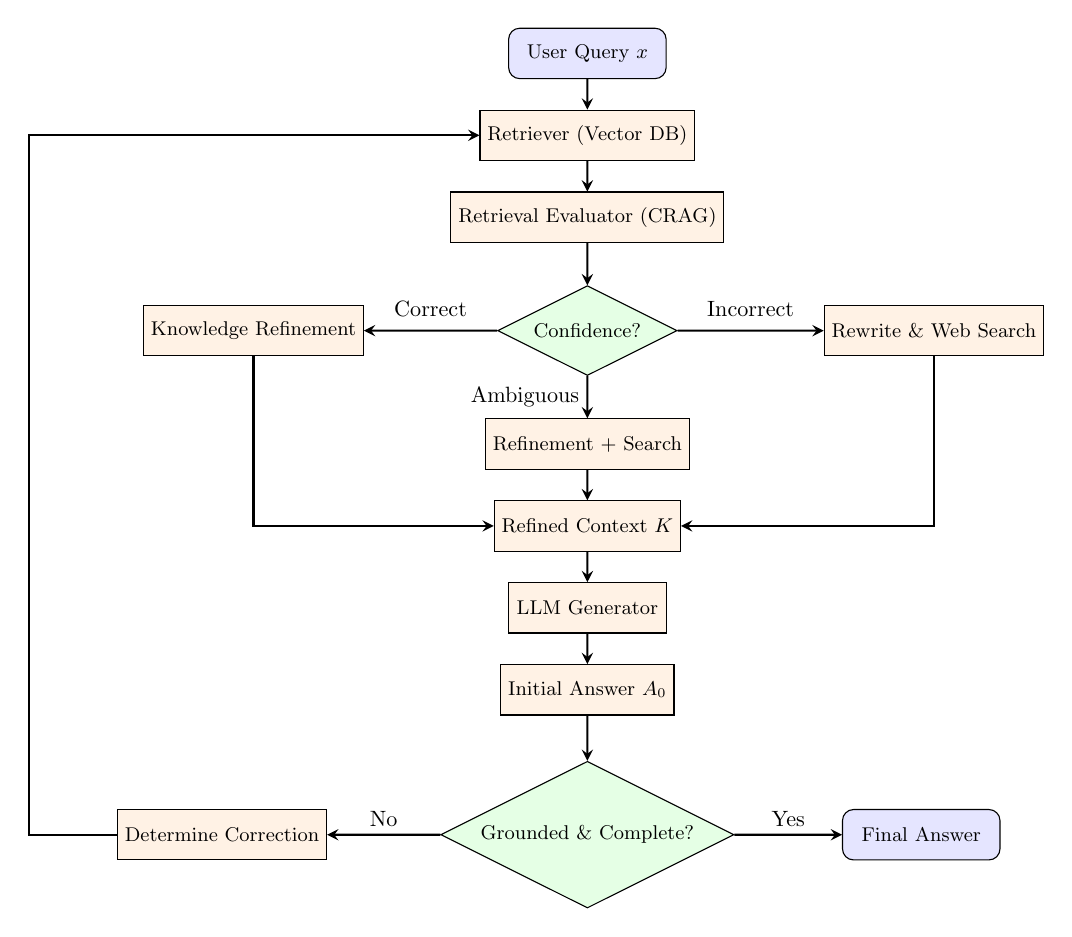
\begin{tikzpicture}[node distance=1.3cm, scale=0.8, every node/.style={transform shape}]
        % Nodes
        \node (query) [startstop] {User Query $x$};
        \node (retriever) [process, below of=query] {Retriever (Vector DB)};
        \node (evaluator) [process, below of=retriever] {Retrieval Evaluator (CRAG)};
        \node (decision) [decision, below of=evaluator, yshift=-0.5cm] {Confidence?};
        
        \node (refinement) [process, left of=decision, xshift=-4cm] {Knowledge Refinement};
        \node (search) [process, right of=decision, xshift=4.2cm] {Rewrite \& Web Search};
        \node (ambiguous) [process, below of=decision, yshift=-0.5cm] {Refinement + Search};
        
        \node (context) [process, below of=ambiguous] {Refined Context $K$};
        \node (generator) [process, below of=context] {LLM Generator};
        \node (initial) [process, below of=generator] {Initial Answer $A_0$};
        \node (selfeval) [decision, below of=initial, yshift=-1cm] {Grounded \& Complete?};
        
        \node (final) [startstop, right of=selfeval, xshift=4cm] {Final Answer};
        \node (corrective) [process, left of=selfeval, xshift=-4.5cm] {Determine Correction};
        
        % Connections
        \draw [arrow] (query) -- (retriever);
        \draw [arrow] (retriever) -- (evaluator);
        \draw [arrow] (evaluator) -- (decision);
        
        \draw [arrow] (decision) -- node[anchor=south, yshift=0.1cm] {Correct} (refinement);
        \draw [arrow] (decision) -- node[anchor=south, yshift=0.1cm] {Incorrect} (search);
        \draw [arrow] (decision) -- node[anchor=east] {Ambiguous} (ambiguous);
        
        \draw [arrow] (refinement) |- (context);
        \draw [arrow] (search) |- (context);
        \draw [arrow] (ambiguous) -- (context);
        
        \draw [arrow] (context) -- (generator);
        \draw [arrow] (generator) -- (initial);
        \draw [arrow] (initial) -- (selfeval);
        
        \draw [arrow] (selfeval) -- node[anchor=south] {Yes} (final);
        \draw [arrow] (selfeval) -- node[anchor=south] {No} (corrective);
        
        \draw [arrow] (corrective.west) -- ++(-1.4,0) |- (retriever.west);
    \end{tikzpicture}
    \caption{Proposed Self-Correcting RAG System Architecture.}
    \label{fig:architecture}
\end{figure}

\pagebreak

%===========================================================
% 7. USE CASE DIAGRAM
%===========================================================
\section{Use Case Diagram}
The Use Case Diagram defines the interactions between the external actors (User, Administrator) and the Self-Correcting RAG system. The diagram is illustrated in Figure \ref{fig:usecase}.

\begin{figure}[h!]
    \centering
    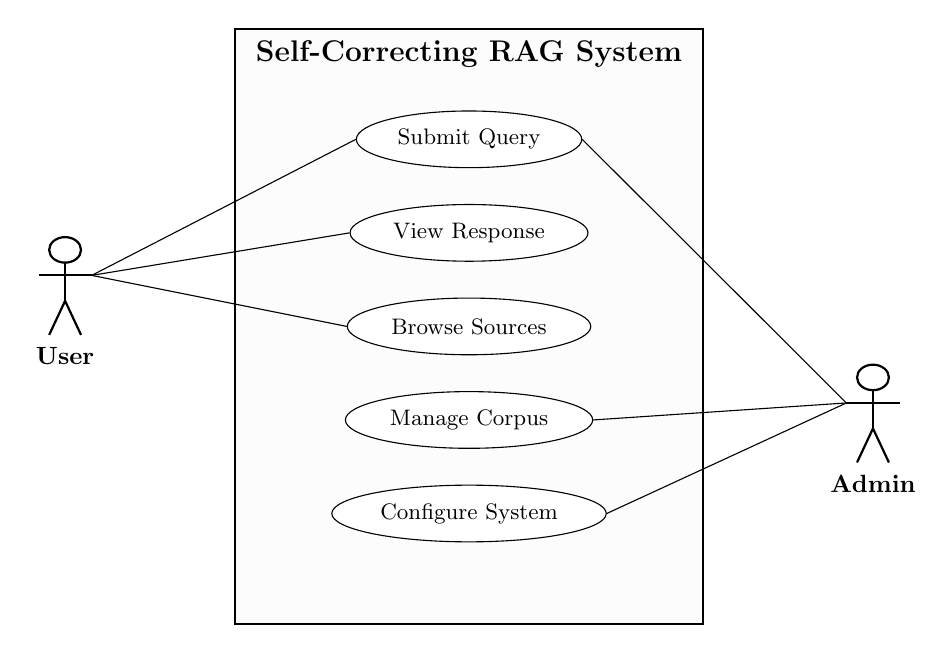
\begin{tikzpicture}[x=1.5cm, y=1.2cm, >=stealth, scale=0.9, every node/.style={transform shape}]
        % System boundary
        \draw[thick, fill=gray!2] (-2.2, -3.5) rectangle (2.2, 3.5);
        \node at (0, 3.2) [font=\large\bfseries] {Self-Correcting RAG System};
        
        % Use Cases
        \node (uc1) [draw, ellipse, minimum width=2.8cm, minimum height=0.8cm, fill=white, align=center] at (0, 2.2) {\small Submit Query};
        \node (uc2) [draw, ellipse, minimum width=2.8cm, minimum height=0.8cm, fill=white, align=center] at (0, 1.1) {\small View Response};
        \node (uc3) [draw, ellipse, minimum width=2.8cm, minimum height=0.8cm, fill=white, align=center] at (0, 0.0) {\small Browse Sources};
        \node (uc4) [draw, ellipse, minimum width=2.8cm, minimum height=0.8cm, fill=white, align=center] at (0, -1.1) {\small Manage Corpus};
        \node (uc5) [draw, ellipse, minimum width=2.8cm, minimum height=0.8cm, fill=white, align=center] at (0, -2.2) {\small Configure System};
        
        % Left Actor: User
        \begin{scope}[shift={(-3.8, 0.5)}]
            \draw[thick] (0,0.4) circle (0.15); % head
            \draw[thick] (0,0.25) -- (0,-0.2); % body
            \draw[thick] (-0.25,0.1) -- (0.25,0.1); % arms
            \draw[thick] (0,-0.2) -- (-0.15,-0.6); % left leg
            \draw[thick] (0,-0.2) -- (0.15,-0.6); % right leg
            \node at (0,-0.85) [font=\bfseries] {User};
            \coordinate (user) at (0.25, 0.1);
        \end{scope}
        
        % Right Actor: Admin
        \begin{scope}[shift={(3.8, -1.0)}]
            \draw[thick] (0,0.4) circle (0.15); % head
            \draw[thick] (0,0.25) -- (0,-0.2); % body
            \draw[thick] (-0.25,0.1) -- (0.25,0.1); % arms
            \draw[thick] (0,-0.2) -- (-0.15,-0.6); % left leg
            \draw[thick] (0,-0.2) -- (0.15,-0.6); % right leg
            \node at (0,-0.85) [font=\bfseries] {Admin};
            \coordinate (admin) at (-0.25, 0.1);
        \end{scope}
        
        % Connections
        \draw (user) -- (uc1.west);
        \draw (user) -- (uc2.west);
        \draw (user) -- (uc3.west);
        
        \draw (admin) -- (uc4.east);
        \draw (admin) -- (uc5.east);
        \draw (admin) -- (uc1.east); 
    \end{tikzpicture}
    \caption{Use Case Diagram.}
    \label{fig:usecase}
\end{figure}

The User primarily interacts with the query interfaces, while the Administrator configures vector database schemas, uploads reference files, and sets confidence scores for evaluation.

\newpage

%===========================================================
% 8. SEQUENCE DIAGRAM
%===========================================================
\section{Sequence Diagram}
The Sequence Diagram depicts the detailed step-by-step transaction flow and temporal execution between the User, Orchestrator, Retriever, Evaluator, Web Search API, Generator, and Critique modules. The process is shown in Figure \ref{fig:sequence}.

% TODO fix this diagram, make it more extensive
\begin{figure}[h!]
    \centering
    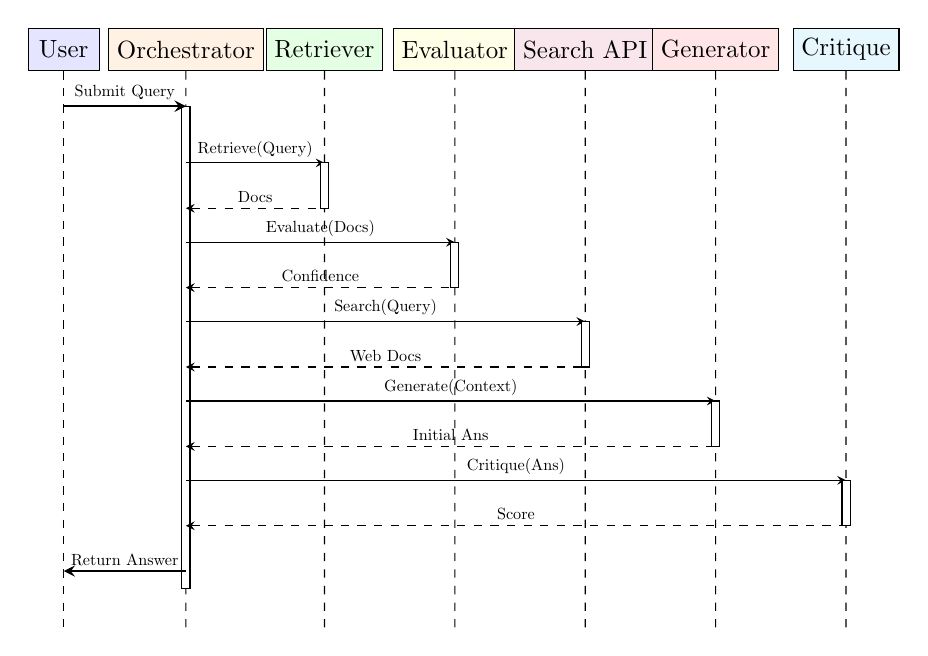
\begin{tikzpicture}[x=1.15cm, y=-0.8cm, >=stealth, scale=0.9, every node/.style={transform shape}]
        % Participants
        \node (user) at (0,0) [draw, fill=blue!10, minimum width=1.0cm, minimum height=0.6cm] {User};
        \node (orch) at (1.5,0) [draw, fill=orange!10, minimum width=1.2cm, minimum height=0.6cm] {Orchestrator};
        \node (ret) at (3.2,0) [draw, fill=green!10, minimum width=1.0cm, minimum height=0.6cm] {Retriever};
        \node (eval) at (4.8,0) [draw, fill=yellow!10, minimum width=1.0cm, minimum height=0.6cm] {Evaluator};
        \node (search) at (6.4,0) [draw, fill=purple!10, minimum width=1.0cm, minimum height=0.6cm] {Search API};
        \node (gen) at (8.0,0) [draw, fill=red!10, minimum width=1.0cm, minimum height=0.6cm] {Generator};
        \node (crit) at (9.6,0) [draw, fill=cyan!10, minimum width=1.0cm, minimum height=0.6cm] {Critique};
        
        % Lifelines
        \draw[dashed] (user) -- (0,10.2);
        \draw[dashed] (orch) -- (1.5,10.2);
        \draw[dashed] (ret) -- (3.2,10.2);
        \draw[dashed] (eval) -- (4.8,10.2);
        \draw[dashed] (search) -- (6.4,10.2);
        \draw[dashed] (gen) -- (8.0,10.2);
        \draw[dashed] (crit) -- (9.6,10.2);
        
        % Activations
        \draw[fill=white] (1.45,1) rectangle (1.55,9.5);
        
        % Message Arrows
        \draw[->, thick] (0,1) -- node[above, scale=0.65] {Submit Query} (1.5,1);
        
        \draw[->] (1.5,2) -- node[above, scale=0.65] {Retrieve(Query)} (3.2,2);
        \draw[fill=white] (3.15,2) rectangle (3.25,2.8);
        \draw[<-, dashed] (1.5,2.8) -- node[above, scale=0.65] {Docs} (3.2,2.8);
        
        \draw[->] (1.5,3.4) -- node[above, scale=0.65] {Evaluate(Docs)} (4.8,3.4);
        \draw[fill=white] (4.75,3.4) rectangle (4.85,4.2);
        \draw[<-, dashed] (1.5,4.2) -- node[above, scale=0.65] {Confidence} (4.8,4.2);
        
        \draw[->] (1.5,4.8) -- node[above, scale=0.65] {Search(Query)} (6.4,4.8);
        \draw[fill=white] (6.35,4.8) rectangle (6.45,5.6);
        \draw[<-, dashed] (1.5,5.6) -- node[above, scale=0.65] {Web Docs} (6.4,5.6);
        
        \draw[->] (1.5,6.2) -- node[above, scale=0.65] {Generate(Context)} (8.0,6.2);
        \draw[fill=white] (7.95,6.2) rectangle (8.05,7.0);
        \draw[<-, dashed] (1.5,7.0) -- node[above, scale=0.65] {Initial Ans} (8.0,7.0);
        
        \draw[->] (1.5,7.6) -- node[above, scale=0.65] {Critique(Ans)} (9.6,7.6);
        \draw[fill=white] (9.55,7.6) rectangle (9.65,8.4);
        \draw[<-, dashed] (1.5,8.4) -- node[above, scale=0.65] {Score} (9.6,8.4);
        
        \draw[->, thick] (1.5,9.2) -- node[above, scale=0.65] {Return Answer} (0,9.2);
    \end{tikzpicture}
    \caption{Sequence Diagram.}
    \label{fig:sequence}
\end{figure}

\newpage

%===========================================================
% 9. DATA FLOW DIAGRAM
%===========================================================
\section{Data Flow Diagram}

\subsection{Level 0 DFD (Context Diagram)}
The Context Diagram (Figure \ref{fig:dfd0}) outlines the scope of the system by illustrating the boundaries and external entities that supply information to, or consume outputs from, the RAG system.

\begin{figure}[h!]
    \centering
    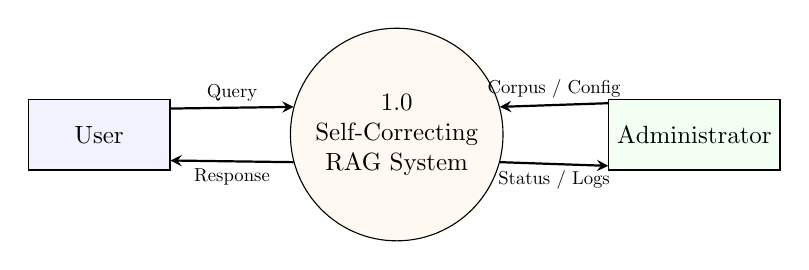
\begin{tikzpicture}[node distance=2.5cm, >=stealth, scale=0.9, every node/.style={transform shape}]
        % Entities
        \node (user) [draw, rectangle, minimum width=2cm, minimum height=1cm, fill=blue!5] {User};
        \node (system) [draw, circle, minimum width=3cm, minimum height=3cm, fill=orange!5, align=center] at (4.2, 0) {1.0\\Self-Correcting\\RAG System};
        \node (admin) [draw, rectangle, minimum width=2cm, minimum height=1cm, fill=green!5] at (8.4, 0) {Administrator};
        
        % Flows
        \draw[->, thick] (user.20) -- node[above, scale=0.75] {Query} (system.165);
        \draw[<-, thick] (user.340) -- node[below, scale=0.75] {Response} (system.195);
        
        \draw[->, thick] (admin.160) -- node[above, scale=0.75] {Corpus / Config} (system.15);
        \draw[<-, thick] (admin.200) -- node[below, scale=0.75] {Status / Logs} (system.345);
    \end{tikzpicture}
    \caption{Level 0 DFD (Context Diagram).}
    \label{fig:dfd0}
\end{figure}

\subsection{Level 1 DFD}
The Level 1 Data Flow Diagram (Figure \ref{fig:dfd1}) details the sub-processes responsible for document retrieval, confidence evaluation, web scraping fallback, context assembly, response generation, and post-generation reflection.

\begin{figure}[h!]
    \centering
    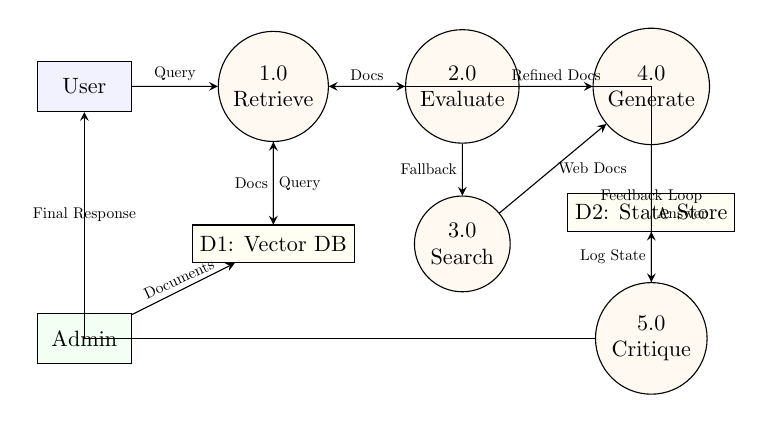
\begin{tikzpicture}[node distance=2.2cm, >=stealth, scale=0.8, every node/.style={transform shape}]
        % External Entities
        \node (user) [draw, rectangle, minimum width=1.5cm, minimum height=0.8cm, fill=blue!5] at (0, 2) {User};
        \node (admin) [draw, rectangle, minimum width=1.5cm, minimum height=0.8cm, fill=green!5] at (0, -2) {Admin};
        
        % Processes
        \node (p1) [draw, circle, minimum width=1.5cm, fill=orange!5, align=center] at (3, 2) {1.0\\Retrieve};
        \node (p2) [draw, circle, minimum width=1.5cm, fill=orange!5, align=center] at (6, 2) {2.0\\Evaluate};
        \node (p3) [draw, circle, minimum width=1.5cm, fill=orange!5, align=center] at (6, -0.5) {3.0\\Search};
        \node (p4) [draw, circle, minimum width=1.5cm, fill=orange!5, align=center] at (9, 2) {4.0\\Generate};
        \node (p5) [draw, circle, minimum width=1.5cm, fill=orange!5, align=center] at (9, -2) {5.0\\Critique};
        
        % Data Stores
        \node (ds1) [draw, rectangle, minimum width=2.2cm, minimum height=0.6cm, fill=yellow!5, align=left] at (3, -0.5) {D1: Vector DB};
        \node (ds2) [draw, rectangle, minimum width=2.2cm, minimum height=0.6cm, fill=yellow!5, align=left] at (9, 0) {D2: State Store};
        
        % Flows
        \draw[->] (user) -- node[above, scale=0.7] {Query} (p1);
        \draw[->] (admin) -- node[above, scale=0.7, rotate=25] {Documents} (ds1);
        
        \draw[->] (p1) -- node[right, scale=0.7] {Query} (ds1);
        \draw[<-] (p1) -- node[left, scale=0.7] {Docs} (ds1);
        
        \draw[->] (p1) -- node[above, scale=0.7] {Docs} (p2);
        \draw[->] (p2) -- node[above, scale=0.7] {Refined Docs} (p4);
        \draw[->] (p2) -- node[left, scale=0.7] {Fallback} (p3);
        \draw[->] (p3) -- node[right, scale=0.7] {Web Docs} (p4);
        
        \draw[->] (p4) -- node[right, scale=0.7] {Answer} (p5);
        \draw[->] (p5) -- node[left, scale=0.7] {Log State} (ds2);
        \draw[->] (p5) |- node[below, pos=0.25, scale=0.7] {Feedback Loop} (p1);
        
        \draw[->] (p5) -| node[below, pos=0.8, scale=0.7] {Final Response} (user);
    \end{tikzpicture}
    \caption{Level 1 DFD.}
    \label{fig:dfd1}
\end{figure}

\newpage

%===========================================================
% 10. ER-DIAGRAM
%===========================================================
\section{Entity Relationship Diagram (ERD)}
To track the state of conversations, documents, system logs, evaluations, and web cache, a database schema is implemented. Figure \ref{fig:er} models this structure.

\begin{figure}[h!]
    \centering
    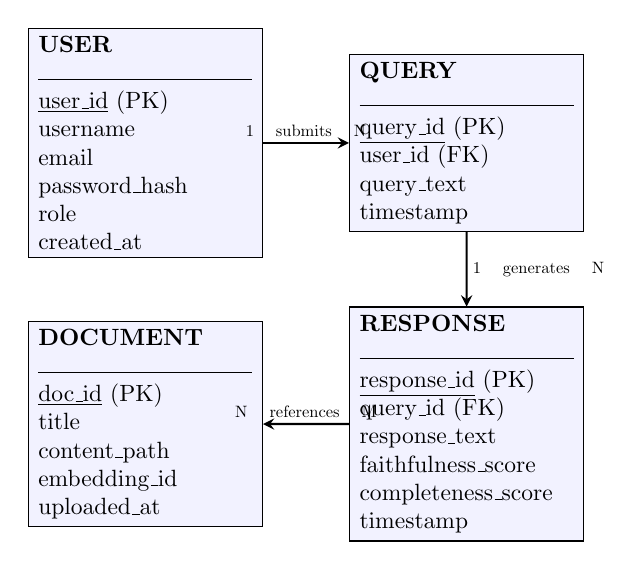
\begin{tikzpicture}[node distance=3cm, >=stealth, scale=0.85, every node/.style={transform shape}]
        % User Table
        \node (user) [draw, rectangle, fill=blue!5, minimum width=3.5cm, align=left] {
            \textbf{USER} \\
            \rule{3.2cm}{0.4pt} \\
            \underline{user\_id} (PK) \\
            username \\
            email \\
            password\_hash \\
            role \\
            created\_at
        };
        
        % Query Table
        \node (query) [draw, rectangle, fill=blue!5, minimum width=3.5cm, align=left, right of=user, xshift=1.8cm] {
            \textbf{QUERY} \\
            \rule{3.2cm}{0.4pt} \\
            \underline{query\_id} (PK) \\
            user\_id (FK) \\
            query\_text \\
            timestamp
        };
        
        % Response Table
        \node (resp) [draw, rectangle, fill=blue!5, minimum width=3.5cm, align=left, below of=query, yshift=-1.2cm] {
            \textbf{RESPONSE} \\
            \rule{3.2cm}{0.4pt} \\
            \underline{response\_id} (PK) \\
            query\_id (FK) \\
            response\_text \\
            faithfulness\_score \\
            completeness\_score \\
            timestamp
        };
        
        % Document Table
        \node (doc) [draw, rectangle, fill=blue!5, minimum width=3.5cm, align=left, left of=resp, xshift=-1.8cm] {
            \textbf{DOCUMENT} \\
            \rule{3.2cm}{0.4pt} \\
            \underline{doc\_id} (PK) \\
            title \\
            content\_path \\
            embedding\_id \\
            uploaded\_at
        };
        
        % Connections
        \draw[->, thick] (user.east) -- node[above, scale=0.7] {1 \quad submits \quad N} (query.west);
        \draw[->, thick] (query.south) -- node[right, scale=0.7] {1 \quad generates \quad N} (resp.north);
        \draw[->, thick] (resp.west) -- node[above, scale=0.7] {N \quad references \quad M} (doc.east);
    \end{tikzpicture}
    \caption{Entity Relationship Diagram.}
    \label{fig:er}
\end{figure}

\newpage

%===========================================================
% 11. TIME FRAME (GANTT CHART)
%===========================================================
\section{Time Frame (Gantt Chart)}
The project implementation is structured over a 16-week cycle during the final semester. The timeline distribution across key phases is shown in Figure \ref{fig:gantt}.

\begin{figure}[h!]
    \centering
    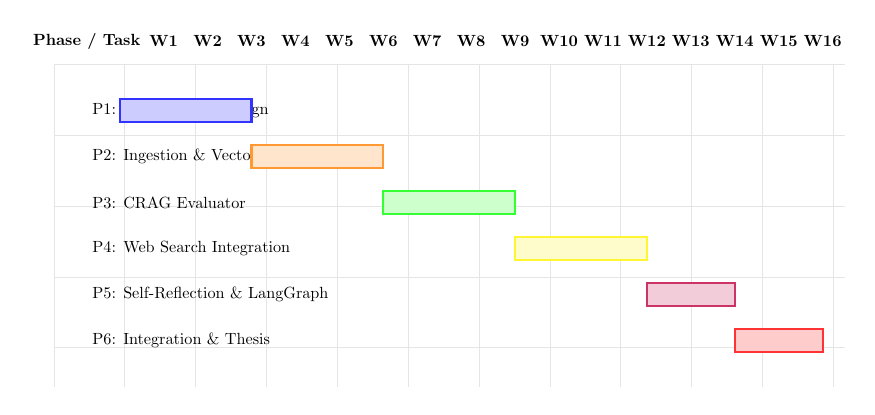
\begin{tikzpicture}[x=0.62cm, y=-0.65cm, >=stealth, scale=0.9, every node/.style={transform shape}]
        % Draw Grid
        \draw[gray!20, very thin] (0,0) grid (18, 7);
        
        % Week Headers
        \foreach \w in {1,...,16} {
            \node at (\w+1.5, -0.5) [scale=0.65, font=\bfseries] {W\w};
        }
        \node at (0.75, -0.5) [scale=0.65, font=\bfseries] {Phase / Task};
        
        % Phase Labels
        \node at (0.75, 1) [scale=0.65, align=left, anchor=west] {P1: Lit Survey \& Design};
        \node at (0.75, 2) [scale=0.65, align=left, anchor=west] {P2: Ingestion \& Vector DB};
        \node at (0.75, 3) [scale=0.65, align=left, anchor=west] {P3: CRAG Evaluator};
        \node at (0.75, 4) [scale=0.65, align=left, anchor=west] {P4: Web Search Integration};
        \node at (0.75, 5) [scale=0.65, align=left, anchor=west] {P5: Self-Reflection \& LangGraph};
        \node at (0.75, 6) [scale=0.65, align=left, anchor=west] {P6: Integration \& Thesis};
        
        % Gantt Bars
        \draw[fill=blue!20, draw=blue!80, thick] (1.5, 0.75) rectangle (4.5, 1.25);   % Weeks 1-3
        \draw[fill=orange!20, draw=orange!80, thick] (4.5, 1.75) rectangle (7.5, 2.25); % Weeks 4-6
        \draw[fill=green!20, draw=green!80, thick] (7.5, 2.75) rectangle (10.5, 3.25); % Weeks 7-9
        \draw[fill=yellow!20, draw=yellow!80, thick] (10.5, 3.75) rectangle (13.5, 4.25); % Weeks 10-12
        \draw[fill=purple!20, draw=purple!80, thick] (13.5, 4.75) rectangle (15.5, 5.25); % Weeks 13-14
        \draw[fill=red!20, draw=red!80, thick] (15.5, 5.75) rectangle (17.5, 6.25);   % Weeks 15-16
    \end{tikzpicture}
    \caption{Project Gantt Chart Timeline.}
    \label{fig:gantt}
\end{figure}

\newpage

%===========================================================
% 12. REFERENCES
%===========================================================
\begin{thebibliography}{99}
\addcontentsline{toc}{section}{References}

\bibitem{crag}
Shi-Qi Yan, Jia-Chen Gu, Yun Zhu, and Zhen-Hua Ling.
\newblock Corrective Retrieval Augmented Generation.
\newblock {\em arXiv preprint arXiv:2401.15884}, 2024.

\bibitem{selfrag}
Akari Asai, Zeqiu Wu, Yizhong Wang, Avirup Sil, and Hannaneh Hajishirzi.
\newblock Self-RAG: Learning to retrieve, generate, and critique through self-reflection.
\newblock In {\em International Conference on Learning Representations (ICLR)}, 2024.

\bibitem{rag}
Patrick Lewis, Ethan Perez, Aleksandra Piktus, Fabio Petroni, Vladimir Karpukhin, Naman Goyal, Heinrich K{\"u}ttler, Mike Lewis, Wen-tau Yih, Tim Rockt{\"a}schel, Sebastian Riedel, and Douwe Kiela.
\newblock Retrieval-augmented generation for knowledge-intensive NLP tasks.
\newblock {\em Advances in Neural Information Processing Systems}, 33:9459--9474, 2020.

\bibitem{hallucination}
Ziwei Ji, Nayeon Lee, Rita Frieske, Tiezheng Yu, Dan Su, Yan Xu, Etsuko Ishii, Yejin Bang, Andrea Madotto, and Pascale Fung.
\newblock Survey of hallucination in natural language generation.
\newblock {\em ACM Computing Surveys (CSUR)}, 55(12):1--38, 2023.

\bibitem{langgraph}
Harrison Chase.
\newblock LangGraph: Building language agents as graphs.
\newblock {\em LangChain Blog}, 2024.

\end{thebibliography}

\end{document}
